\documentclass{standalone}
\usepackage{tikz}
\usetikzlibrary{shapes,arrows,positioning}
\begin{document}
  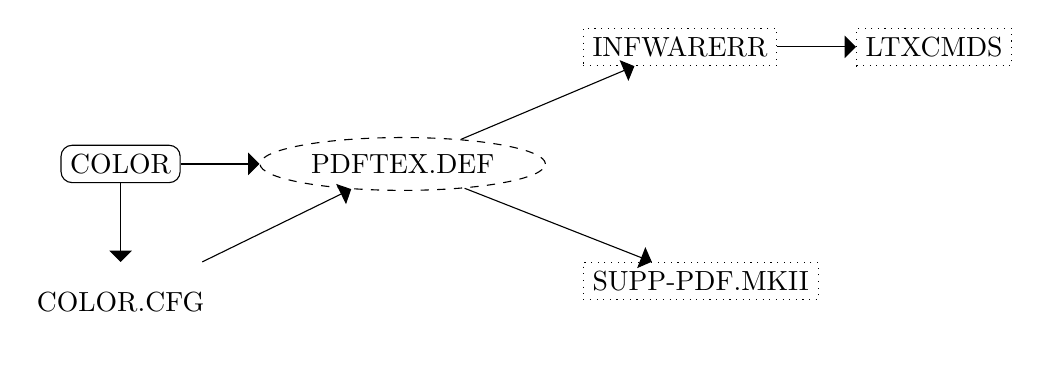
\begin{tikzpicture}
  
  \tikzset{main node/.style={rectangle, draw,
  		text centered, rounded corners}, }
  \tikzset{driver node/.style={ellipse, draw,dashed,
  		text centered}, }
   \tikzset{fmt node/.style={rectangle, draw,dotted,
   		text centered}, }
  \tikzset{cfg node/.style={minimum size=1cm}, }
  \tikzset{linea/.style={-triangle 90}, }
\node[main node] (1)   {COLOR};
\node[cfg node] (2)[below =of 1]   {COLOR.CFG};
\node[driver node] (3)[right =of 1]   {PDFTEX.DEF};
\node[fmt node] (4)[above right =of 3]   {INFWARERR};
\node[fmt node] (5)[below right =of 3]   {SUPP-PDF.MKII};
\node[fmt node] (6)[right =of 4]   {LTXCMDS};
\foreach \x /\y in{1/2,1/3,2/3,3/5,3/4,4/6}
  \path[linea] (\x) edge node {} (\y);
%%  
\end{tikzpicture}
\end{document}